% %%%%%%%%%%%%%%%%%%%%%%%%%%%%%%%%%%%%%%%%%%%%%%%%%%%%%%%%%%%%%%%%%%%%%
% %% State-of-the-Art %%
% SpArch
% %%%%%%%%%%%%%%%%%%%%%%%%%%%%%%%%%%%%%%%%%%%%%%%%%%%%%%%%%%%%%%%%%%%%%

\subsection{SpArch}
\label{sec:soa:sparch}

SpArch~\cite{Zhekai2020_SpArch} uses an \algo{OP} algorithm for SpGEMM in order to benefit from the simplified access pattern for the inputs. To address the management of the large volume of \emph{POs}, SpArch  pipelines the \emph{multiply} and \emph{merge} phases and uses condensing methods to reduce the number of \emph{POs} and scheduling methods to reduce memory traffic.
Unlike other \algo{OP} accelerators~\cite{Pal2018_OuterSPACE}, with SpArch, both $A$ and $B$ are stored in \emph{(UOP, CP) row-major} format. As a consequence of this \emph{CSR} format, the $A$-rows can easily be condensed to the left (see Figure~\ref{fig:soa:sparch_algo}). Thus, when a condensed $A$-column is read, it will require reading all the $B$-rows corresponding to the different $A$-columns that have been combined. The \emph{MatA Column Fetcher} reads the combined $A$-columns and the \emph{MatB Row Prefetcher} reads the necessary $B$-rows (see Figure~\ref{fig:soa:sparch}), thus masking the memory latency. The \emph{MatB Row Prefetcher}, stores multiple $B$-rows in a cache, and it uses information about the upcoming $A$-columns  (provided by the \emph{Distance List Builder}) to ensure the needed $B$-rows are kept in the cache.

A key contribution of SpArch is the merge unit that is able to merge sixty-four \emph{POs} in parallel, through a binary tree type architecture. The core of the merger is a brick which compares and merges 4$\times$4 $(index, value)$ pairs in one cycle. These are combined to build a hierarchical merger array whose output is then written to main memory, and read back for further merging by the \emph{Partial Matrix Fetcher}. The authors note that the order in which the \emph{reductions} are performed is important, specifically sparser \emph{POs} should be merged first and they propose a Huffman tree scheduler to determine the best order to minimize memory accesses.
Overall, SpArch is able to compute an \algo{OP} SpGEMM\footnote{Since the merger can read \emph{POs} from memory, the $D$-matrix can be treated like an initial \emph{PO}.} kernel with reduced main memory traffic for the \emph{POs} mainly by addressing the \emph{scatter} problem with a highly parallelized merger.

\begin{figure}
    \centering
    \begin{minipage}[b]{0.54\linewidth}
        \begin{figure}[H]
            \centering
            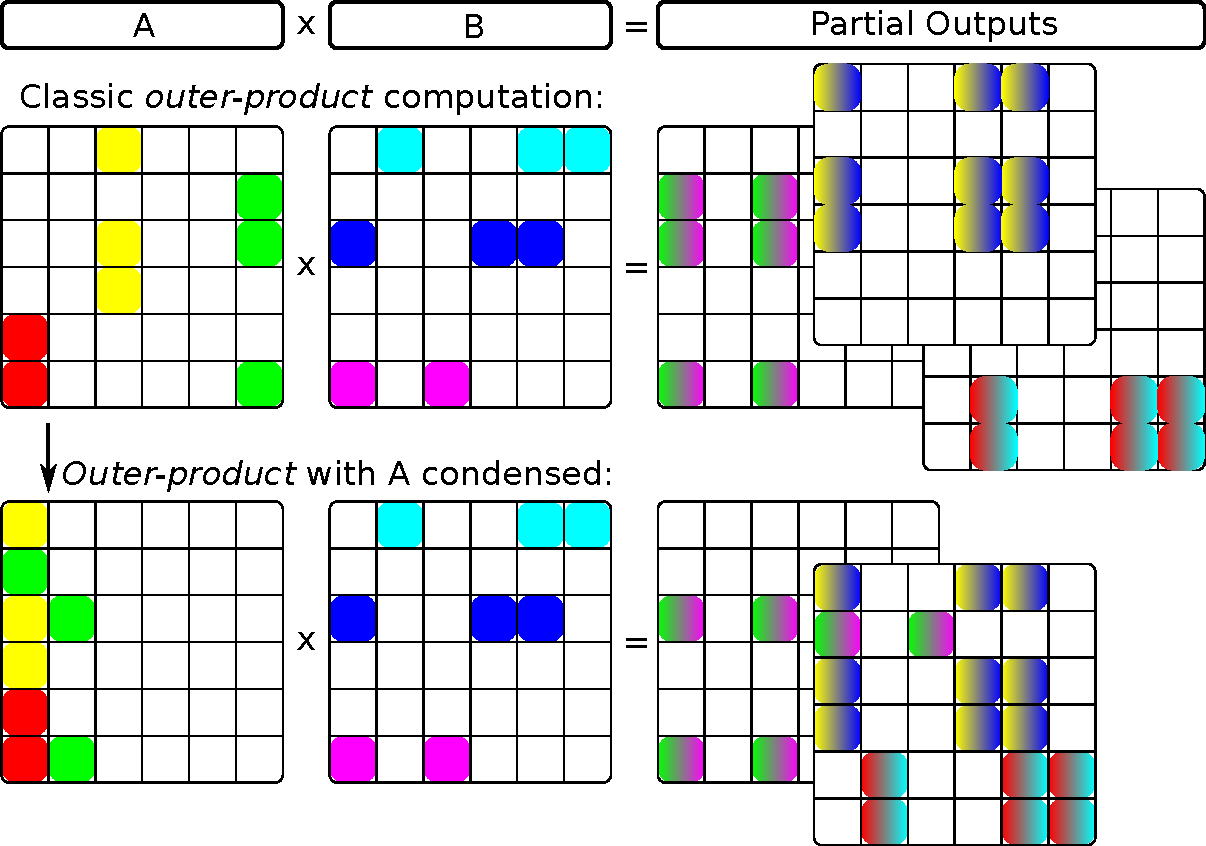
\includegraphics[width=0.85\linewidth]{Chapter_SoA/Figures/PDF/SpArch_algo.pdf}
            \caption{\emph{Outer-product} with a Condense $A$-Matrix}
            \label{fig:soa:sparch_algo}
        \end{figure}
    \end{minipage}
    \hfill
    \begin{minipage}[b]{0.44\linewidth}
        \begin{figure}[H]
            \centering
            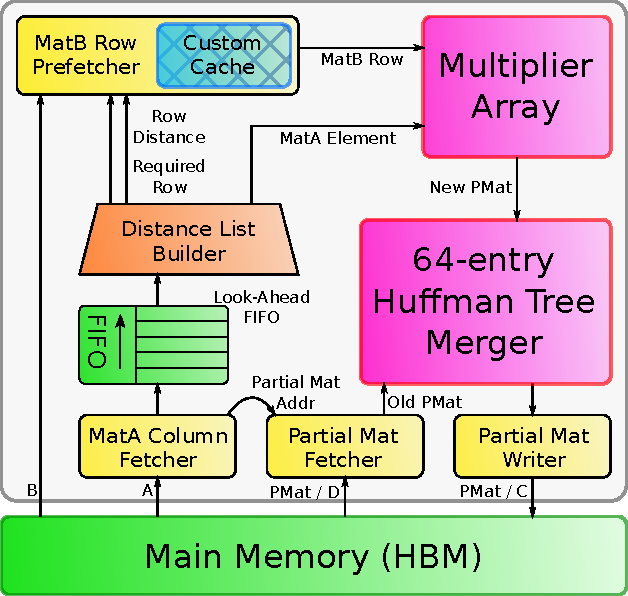
\includegraphics[width=0.8\linewidth]{Chapter_SoA/Figures/PDF/SpArch.pdf}
            \caption{Architecture of SpArch}
            \label{fig:soa:sparch}
        \end{figure}
    \end{minipage}
\end{figure}